%---------------------------------------------------
% Exponential (& Logarithmic) Functions
%---------------------------------------------------
\chapter[Exponential Functions]{Exponential \& Logarithmic \\Functions}
We defined the polynomial $a^{x}$ in chapter 1, however $x$ was restricted to rational numbers. We now want to explore $a^{x}$ where and $x$ is any real number. 

We can show that values exist simply by pressing buttons on the calculator or drawing a graph using \desmos, however an intuitive understanding can be obtained by considering appropriate values. 

Consider $2^{\pi }$. We know $\pi  =3.141592654 \ldots $. $2^{\pi }$ should be between $2^{3}$\ and $2^{4}$. That is between $8$ and $16$. We can evaluate 

\qquad \qquad \qquad \qquad \qquad \qquad \qquad \qquad
\begin{tabular}[c]{ll}$2^{3.1}$  & $8.5741877$  \\
	$2^{3.14}$  & $8.815240927$  \\
	$2^{3.141}$  & $8.821353305$  \\
	$2^{3.1415}$  & $8.824411082$  \\
	$2^{3.14159}$  & $8.824961595$  \\
	$2^{3.141592}$  & $8.824973829$  \\
	$2^{3.1415926}$  & $8.824977499$  \\
	$2^{3.14159265}$  & $8.824977805$  \\
	$2^{3.141592654}$  & $8.82497783$
\end{tabular}

We could continue this process. If we enter $2^{\pi }$ on the calculator the answer obtained is
\begin{equation*}2^{\pi } =8.824977827
\end{equation*}

The graph of $y =2^{x}$ is shown below. Notice it will never go below $y=0$.\\ 
\begin{center}
	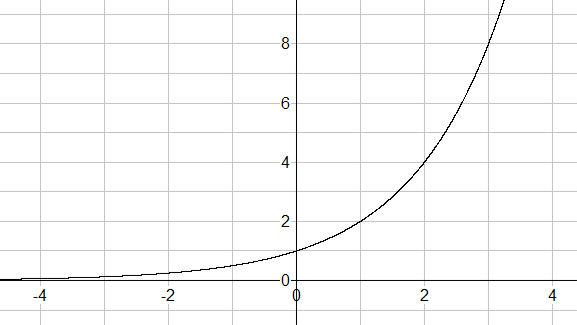
\includegraphics[width=3.7758in, height=2.1378in,]{L4SZ282M}
\end{center}

Recall $y =f (x)$ is a function and $y =f ( -x)$ is the same function with every $x$ replaced with $ -x$, i.e. $y =f ( -x)$ is the reflection of $y =f (x)$ in the $y$-axis. 

If $y =2^{x}$ then $y =2^{ -x}$ is the reflection of $y =2^{x}$ in the $y$-axis. But $y =2^{ -x} =\left (2^{ -1}\right )^{x} =\genfrac{(}{)}{}{}{1}{2}^{x}$. 

\textbf{Graphing Exercise} Use Desmos to verify that $y =2^{-x}$ and $y =\frac{1}{2}^x$ are equivalent. 

\subsection*{The Exponential Function $f(x)=a^x$}
Let $y =a^{x}$ where $a >0$ 

\begin{center}
\begin{tabular}{lcl}
	\toprule
	When $0 <a <1$  & $y =a^{x}$ looks like  &    
	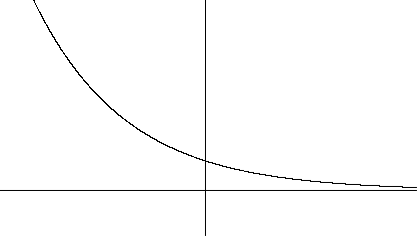
\includegraphics[ width=1.9086in, height=1.0853in,]{L4SZ282O}
	\\
	\midrule
	When $a =1$  & $y =a^{x} =1^{x} =1$ looks like  &    
	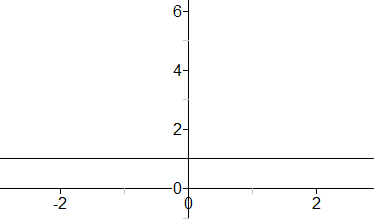
\includegraphics[ width=1.9095in, height=1.1234in,]{L4SZ282P}
	\\
	\midrule
	When $a >1$  & $y =a^{x}$ looks like  &    
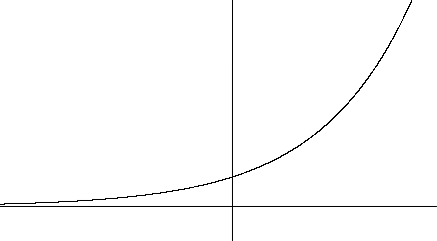
\includegraphics[ width=1.9372in, height=1.0741in,]{L4SZ282Q}
	\\
	\bottomrule
\end{tabular}
\end{center}

$f (x) =a^{x}$ is called an \emph{exponential} function. $a$ is called the \emph{base} of the exponential function. The domain
is $\mathbb{R}$. the range is $\left (0 ,\infty \right )$. The $x$-axis is an asymptote. 

\example Find the equation of the exponential function that passes through $\left (0 ,1\right )$ and $\left (3 ,125\right )$. 

\solution An exponential function that passes through $\left (0 ,1\right )$ is of the form $f (x) =a^{x}$. As $f (3) =125$ we substitute $x =3$ and get
\begin{align*}a^{3} &  = 125 \\
a &  = \sqrt[{3}]{125} =5\\
\therefore f(x)&=5^x \text{ satisfies the conditions.}
\end{align*}

\subsection*{Transformations of Exponential Functions}
Recall the transformations we have met so far:
\begin{center}
\begin{tabular}{ll}Vertical stretch of $a$  & $y =f (x) \leadsto y =a f (x)$  \\
	Horizontal stretch of $\frac{1}{b}$  & $y =f (x) \leadsto y =f (b x)$  \\
	Vertical shift of $c$ $\uparrow $  & $y =f (x) \leadsto y =f (x) +c$  \\
	Horizontal shift of $d$ $ \longrightarrow $  & $y =f (x) \leadsto y =f (x -d)$  \\
	Reflection in $x$-axis  & $y =f (x) \leadsto y = -f (x)$  \\
	Reflection in $y$-axis  & $y =f (x) \leadsto y =f ( -x)$
\end{tabular}
\end{center}
Each of these transformations can be applied to an exponential function. Horizontal shifts are `attached' to the $x$ with brackets and opposite to convention. A shift to the right is represented by negative, e.g., $y=2^(x-3)$. Vertical shifts are positive to shift up and negative to shift down.
\begin{center}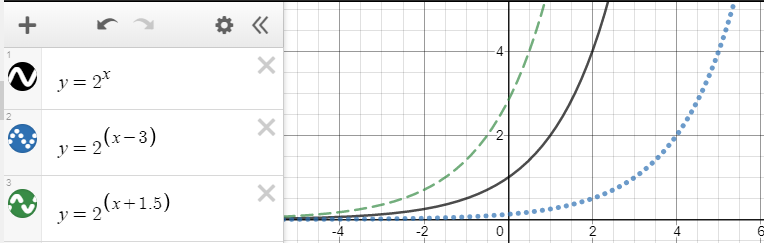
\includegraphics[width=14cm]{expTrans1}\end{center}
Reflections are accomplished by multiplying by negative one. To reflect in the $x$-axis, multiply the whole function by $-1$, e.g., $y=-2^x$. And for a reflection in the $y$-axis multiply the $x$ variable by $-1$, e.g., $y=2^{-x}$.
\begin{center}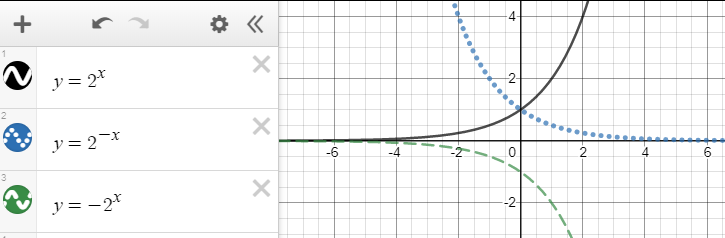
\includegraphics[width=14cm]{expTrans2}\end{center}
See the lecture notes for more examples.
%---------------------------------------------------
% the natural exponential function e^x
%---------------------------------------------------
%\section{\texorpdfstring{$e^x$}{}}
\section[$e^x$]{The Natural Exponential Function}\label{sec:naturalExponential}
The \emph{natural exponential function} has wide application in mathematics engineering. It arises naturally and crops up in applications such as finance, population, radioactivity, charge on a capacitor, and more. We have defined $f (x) =a^x$ and there is a particular value of $a$ that we denote by the letter $e$. It is an irrational number (like $\pi $, $\sqrt{2}$ etc.) and has a button on your calculator. To 10 decimal places it is
\[e \approx 2.7182818285\dots\]
The natural exponential function $f (x) =e^x$ is often simply referred to as \textit{the} exponential function. 

Compound interest can demonstrate an example of  how the value above is found. Imagine a bank that pays 100\% interest on your money. Given an initial deposit of \$1, at the end of year you will receive \$1 in interest payment and have a total of \$2. Compounded interest allows this to happen at intervals smaller than 1 year. If the interest is compounded twice per year, then after 6 months, you will receive 50\% interest and have \$1.50. In the second half of the year you now have an additional \$0.50 available to earn the second half interest. Now, $\$1.50\times50\%=\$0.75$, so at the end of the year you have \$1.50+\$0.75=\$2.25.

Lets say the interest is compounded monthly, then after 1 month you will receive $\frac{1}{12}\times 100\%=8.33\%$ interest for \$1+\$0.0833=\$1.0833. The second month will earn the same rate (8.33\%) on \$1.0833, for a total of \$1.1736. After 12 months, your dollar will now be worth $\$1.00\times\left(1+\frac{1}{12}\right)^{12}=\$2.6130$. 
\begin{center}
\begin{tabular}{cll}
	\toprule
	compounding periods&interest (\$)&total (\$)\\
	\midrule
	1 (yearly)&1.00&2.00\\
	2&1.25&2.25\\
	3&1.3704 &2.3704\\
	4 (quarterly)& 1.4414 & 2.4414 \\
	5& 1.48832 & 2.48832 \\
	6& 1.521626&2.521626\\\midrule
	12 (monthly)& 1.613035&2.613035 \\\midrule
	52 (weekly)&1.692597 &2.692597\\\midrule
	365 (daily)&1.714567 &2.714567\\\midrule
	continuous& 1.718282&\textbf{2.7182818}$...=$\textit{\textbf{e}}\\
	\bottomrule
\end{tabular}
\end{center}

As a function, $f(x)=e^x$, is plotted below:
\begin{center}
	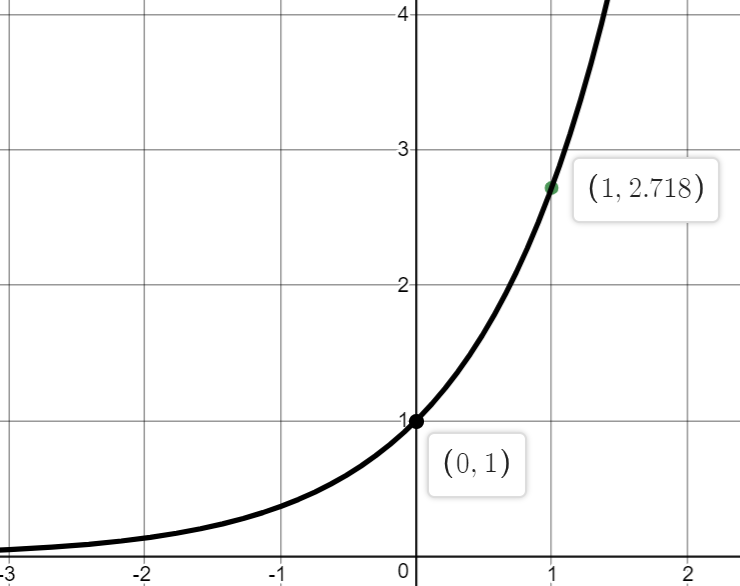
\includegraphics[width=10cm]{exp1}
\end{center}
%---------------------------------------------------
% Logarithmic Functions
%---------------------------------------------------
\section{Logarithmic Functions}
The \emph{logarithmic function} is the inverse of the function $f (x) =a^{x}$. Recall the inverse of a function is the reflection of the function in the line $y =x$. Mathematically this is equivalent to swapping the $x$ and the y in $y =a^{x}$. So $x =a^{y}$ is the inverse of $y =a^{x}$. We have another notation for the inverse of a function, which is a little more complicated. Let $y =f (x)$ be a function of $x$ then $y =f^{ -1} (x)$ is the inverse of this function. 

Sometimes the inverse of the function is also a function. For example the inverse of $y =x^{2}$ is $x =y^{2}$. $y =x^{2}$ is a function (vertical line test always applies), whereas $x =y^{2}$ is not a function (vertical line test is broken). 

\begin{multicols}{2}
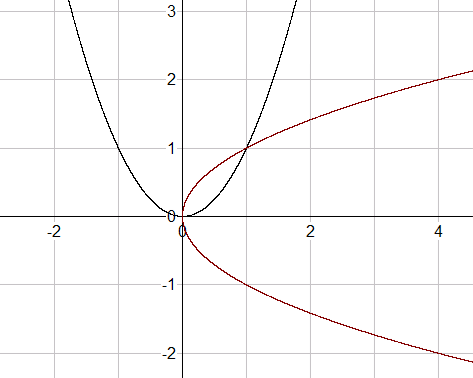
\includegraphics[ width=3.032in, height=2.4275in,]{L4SZ2832}
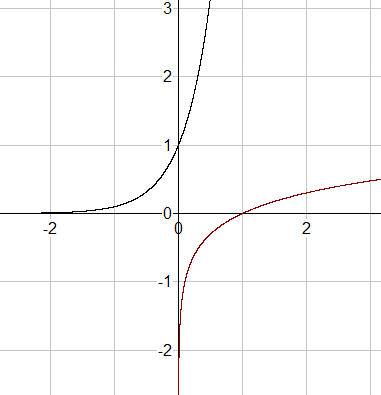
\includegraphics[ width=2.3419in, height=2.4267in,]{L4SZ2833}
\end{multicols}

The inverse of $y =10^{x}$ is $x =10^{y}$. $y =10^{x}$ is a function (vertical line test always applies) and so is $x =10^{y}$. 

Another useful fact to remember about inverses concerns the domain and range. The \emph{domain}
of $f$ is the \emph{range} of $f^{ -1}$ and the \emph{range} of $f$ is the \emph{domain} of $f^{ -1}$. 

We have a notation for $x =a^{y}$ it is $y =\log _{a} x$:
\begin{tcolorbox}
\[y =\log _{a} x \Leftrightarrow x =a^y
\]
\end{tcolorbox}


In $x =a^{y}$ substitute $y =\log _{a} x$ and we get $x =a^{\log _{a} x}$. This means that given a base of $a$ the power (or exponent) to which $a$ must be raised to get $x$ is $\log _{a} x$. 

Problems involving logarithms will often require us to switch back and forth between $y =\log _{a} x$ and $x =a^{y}$, however it is also helpful if you can remember to substitute for $y$ and write $x =a^{\log _{a} x}$ so that you can say ``the logarithm is the power". 

\example
\begin{description}
	\item [(a)] $\log _{10} 100 =2$ because $10^{2} =100$ 
	
	\item [(b)] $\log _{3} 81 =4$ because $3^{4} =81$ 
	
	\item [(c)] $\log _{10} 0.01 = -2$ because $10^{ -2} =0.01$ \end{description}

\subsection*{The graph of $y =\log _{a} x$}
The exponential function $y =a^{x}$ where $a >0$ is now known and its domain is $\mathbb{R}$ and its range is the positive real numbers. We can write $\mathbb{R}^{ +}$, meaning the positive real numbers, instead of $(0 ,\infty)$. 

The graph of $f (x) =a^{x}$ can be reflected in the line $y =x$ and the result is $f^{ -1} (x) =\log _{a} x$. 

\textbf{Graphing Exercise} On the same set of axes draw:
\begin{tasks}(4)
	\task $y =10^{x}$ 
	\task $y =\log _{10} x$ 
	\task $y =x$ 
	\task $x =10^{y}$ 
\end{tasks}

Make a comment about each statement below. 
\begin{tasks}
	\task[1.] Check the graphs in (a), (b) and (c) are you confident that $y =\log _{10} x$ is the reflection of $y =10^{x}$ in the line $y =x$?
	\task[2.] When you enter $x =10^{y}$ describe what takes place.
	\end{tasks}

\textbf{Graphing Exercise Solution} Using \desmos we can see the different plots. Plots (b) and (d) are equivalent, so are on top of each other.\\
\begin{center}
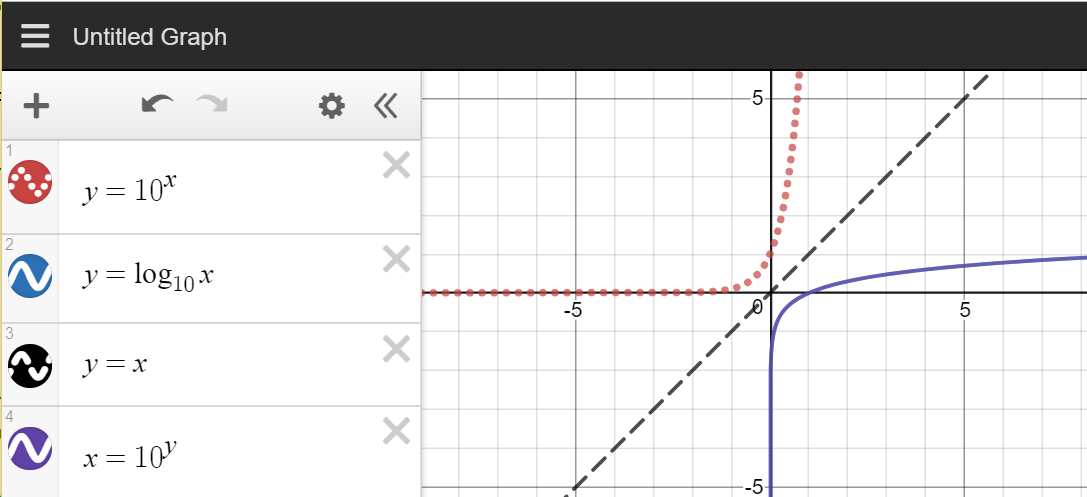
\includegraphics[width=14cm]{logGraph1}\\
\end{center}

\textbf{Graphing Exercise} On the same set of axes draw:
\begin{tasks}(4)
	\task $y =\log _{2} x$ 
	\task $y =\log _{3} x$ 
	\task $y =\log _{4} x$ 
	\task $y =\log _{10} x$ \end{tasks}
\textbf{Graphing Exercise Solution} Using \desmos we can see the relationship between the different bases in the log equation:\\
\begin{center}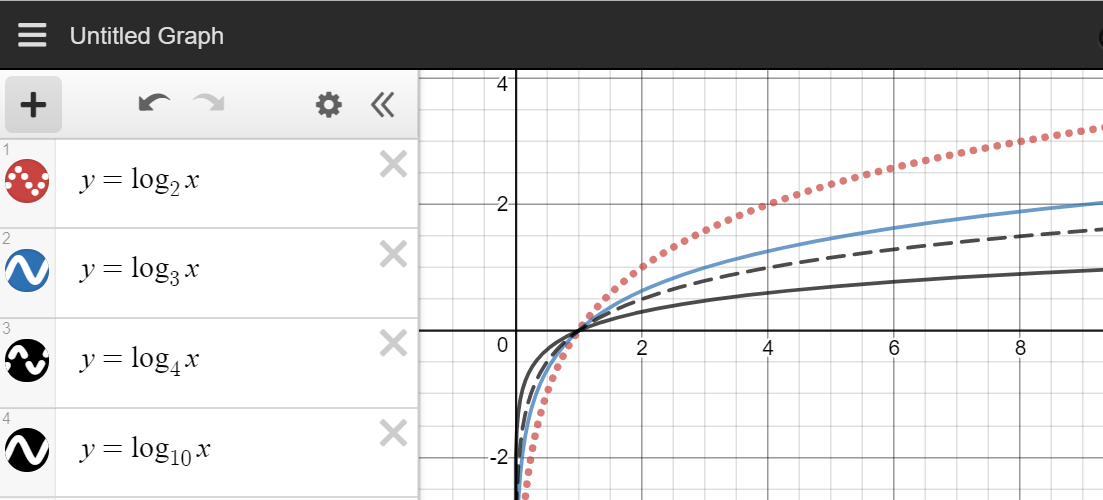
\includegraphics[width=14cm]{logGraph2}\end{center}
Notice the point that is common to all curves and the behaviour of the family of curves for $x >1$ and for $0 <x <1$. 

\textbf{Property 1}: A property of logarithms is $\log _{a} 1 =0$ and this can be seen on the graphs where every graph goes through $\left (1 ,0\right )$. 

The pattern you observe as the base gets bigger might not be evident for values of the base between $0$ and $1$. On the same set of axes draw the following: 

\begin{tasks}(4)
	\task $y =\log _{\frac{1}{2}} x$ 
\task $y =\log _{\frac{1}{3}} x$ 
	\task $y =\log _{\frac{1}{4}} x$ 
	\task $y =\log _{\frac{1}{5}} x$ \end{tasks}
\begin{center}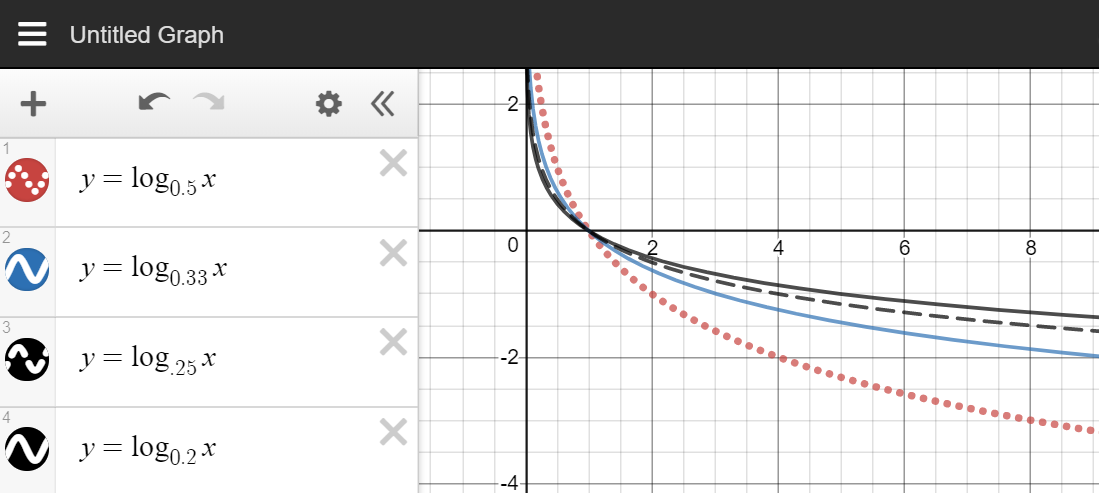
\includegraphics[width=14cm]{logGraph3}\end{center}
To say the pattern is the same you have to be careful to describe the base. Explain how changing the base gives the same pattern as for (a) to (d).

\textbf{Property 2:} A second property of logarithms is $\log _{a} a =1$. That is $a^{1} =a$ or the power to which you have to raise $a$ to get $a$ is $1$. On your curves above locate a point on each curve that shows this. You
should in each case be looking for the point $\left (a ,1\right )$. 

\textbf{Property 3:} A third property
of logarithms is $\log _{a} a^{x} =x$. This useful property must be understood if logarithm problems are to be mastered.
\ You should understand what $\log _{a} a^{x}$ is saying. $a$ is the base so $\log _{a} a^{x} =x$ says ``The power to which $a$ must be raised to get $a^{x}$ is $x$." 

\subsection*{Base-10}
When the base is $10$ we write $y =\log  x$ which \textit{implies} that $y=\log _{10} x$. If you see no base you assume it is base $10$. \Desmos and other mathematics programs recognise ``$\log $'' as being ``logarithm of base $10$.'' The $\log $ key on the calculator gives the base-10 logarithm of any positive number.
\begin{tcolorbox}
\begin{equation*}y =\log  x \Leftrightarrow 10^{y} =x
\end{equation*}
\end{tcolorbox}


\subsection*{Natural Logarithms}
When the base is $e$ we write $y =\log _{e} x =\ln  x$. If you see $\ln  x$ you can assume it is $\log _{e} x$. This is sometimes called the \emph{natural} logarithm of $x$. Software should recognise ``$\ln $'' as meaning ``logarithm to the base $e$.'' The $\ln $ key on the calculator gives the natural logarithm of any positive number.
\begin{tcolorbox}\begin{equation*}y =\ln  x \Leftrightarrow e^{y} =x
\end{equation*}\end{tcolorbox}

\textbf{Graphing Exercise}
Use Desmos to sketch the following. Describe in words how each curve is related to $y =\ln  x$. 

\begin{tasks}(3)
	\task $y =\ln  x$ 
\task  $y =\ln  ( -x)$ 
\task  $y = -\ln  x$ 
	\task  $y =\ln  (x -1)$ 
	\task  $y =\ln  (x) -1$ 
	\task $y =\ln  ( -1 -x)$ \end{tasks}


\section{The Laws of Logarithms}

The logarithmic laws are listed beside their equivalent exponent laws (see Section~\ref{sec:introAlgebra} Exponents) to show the symmetry between the two. The terms \textit{logarithm} and \textit{exponent} are very similar.
\begin{tcolorbox}
\begin{center}
\renewcommand{\arraystretch}{1.2}
\begin{tabular}{lrclcrcl}
	%\toprule
	\multicolumn{4}{c}{Logarithms}& &\multicolumn{3}{c}{Exponents}\\
	\cmidrule{1-4}\cmidrule{6-8}
	Law 1: &$ \log_x(ab) $&$=$&$ \log_x(a)+\log_x(b)  $&\hspace{1cm} &$x^a$&$=$&$x^{a+b} $\\
	Law 2: &$ \log_x\left(\frac{a}{b}\right) $&$=$&$  \log_x(a)-\log_x(b) $& &$\frac{x^a}{x^b}$&$=$&$x^{a-b}  $\\
	Law 3: &$ \log_x(a^b) $&$=$&$ b\cdot\log_x(a)   $& &$(x^a)^b $&$=$&$x^{ab} $\\
	\cmidrule{1-4}\cmidrule{6-8}
	&$  \log_{x}\left(\frac{1}{x^a}\right) $&$=$&$-a   $& &$x^{-a} $&$=$&$\frac{1}{x^a} $\\
	&$ \log_{x}1  $&$=$&$ 0  $& &$x^0 $&$=$&$1 $\\
	&$ \log_x(x) $&$=$&$  1 $& &$x^1 $&$=$&$x $\\
	\bottomrule
	recall:&$ \log_a(x) $&$=$&$y$\hspace{0.5cm} converts to& $\Leftrightarrow$ &$x $&$=$&$a^y $\\
	\bottomrule
\end{tabular}
\end{center}
For all of the above logarithms, $\log_x$ can be replaced with the natural logarithm, $\log_e$,  or $\ln$. So for example:
\begin{center}
	\renewcommand{\arraystretch}{1.2}
	\begin{tabular}{lrcl}
		%\toprule
		Law 1: &$ \ln(ab) $&$=$&$ \ln(a)+\ln(b)  $\\
		Law 2: &$ \ln\left(\frac{a}{b}\right) $&$=$&$  \ln(a)-\ln(b) $\\
		Law 3: &$ \ln(a^b) $&$=$&$ b\cdot\ln(a)$ \\
		%\bottomrule
	\end{tabular}
\end{center}
\end{tcolorbox}
\example
Expand using the logarithm laws 
\begin{description}
	\item [(a)] $\log  \sqrt{3} =\log  3^{\frac{1}{2}} =\frac{1}{2} \log  3$ 
	
	\item [(b)] $\ln  \genfrac{(}{)}{}{}{a \sqrt{b}}{\sqrt[{3}]{c}} =\ln  \left (a b^{\frac{1}{2}} c^{ -\frac{1}{3}}\right ) =\ln  a +\ln  b^{\frac{1}{2}} +\ln  c^{ -\frac{1}{3}} =\ln  a +\frac{1}{2} \ln  b -\frac{1}{3} \ln  c$ \end{description}

\example Evaluate
\begin{description}
	\item [(a)] $\log _{2} 112 -\log _{2} 7 =\log _{2} \frac{112}{7} =\log _{2} 16 =\log _{2} 2^{4} =4 \log _{2} 2 =4$ 
	
	\item [(b)] $\log _{2} 8^{23} =\log _{2} \left (2^{3}\right )^{23} =\log _{2} \left (2^{69}\right ) =69 \log _{2} 2 =69$ 
	
	\item [(c)] $\log  \sqrt{0.001} =\log  \left (0.001\right )^{\frac{1}{2}} =\frac{1}{2} \log  0.001 =\frac{1}{2} \log  10^{ -3} =\frac{1}{2} \times  -3 = -\frac{3}{2} = -1\frac{1}{2}$ 
	
	\item [(d)] $e^{2 \ln  4} =\left (e^{\ln  4}\right )^{2} =4^{2} =16\text{\quad \quad }($Let $\ln  4 =x$ then $e^{x} =4$ so $e^{\ln  x} =4)$ \end{description}

\example Rewrite as a single logarithm term using the logarithm laws 
\begin{description}
	\item [(a)] $\log  12 +\frac{1}{2} \log  5 -\log  3 =\log  \frac{12 \sqrt{5}}{3} =\log  4 \sqrt{5}$ 
	
	\item [(b)] $\log _{3} \left (x^{2} -1\right ) -\log _{3} \left (x -1\right ) =\log _{3} \frac{x^{2} -1}{x -1} =\log _{3} \frac{\left (x +1\right ) \left (x -1\right )}{x -1} =\log _{3} \left (x +1\right )$ \end{description}



%---------------------------------------------------
% Exponential and Logarithmic Equations
%---------------------------------------------------
\section{Exponential and Logarithmic Equations}
The types of problems we meet in this section will be able to be rearranged so that they look like
\begin{equation*}a^{f (x)} =b
\end{equation*}
Where $a$ and $b$ are real numbers, $x$ is the unknown variable we are trying to find and $f (x)$ is an expression in $x$. The technique we will use will be the same for every problem we solve. 

\begin{description}
	\item [Step 1] Our first step is to inspect the problem to see if the unknown
	variable is in the exponent. 
	
	\item [Step 2] Now that we have
	established that we are solving an exponential equation we rearrange it until it is in the form $a^{f (x)} =b$ 
	
	\item [Step 3] Take the logarithm
	of both sides. In most practical situations we either take logarithms to the base $10$ or logarithms to the base $e$. there are three situations 
	
	\item [Case
	1] The problem has reduced to $10^{f (x)} =b$. Take logarithms to the base $10$. 
	
	\item [Case 2] The problem has
	reduced to $e^{f (x)} =b$. Take logarithms to the base $e$. 
	
	\item [Case 3] The problem has
	reduced to $a^{f (x)} =b$ where $a$ is neither $10$ nor $e$. You can take logarithms to the base $10$ or $e$ as you wish, either is correct. 
	
	\item [Step 4]
	Solve the equation you obtain. \end{description}

\textbf{Example 1} Solve $3^{x} =5$. This is an example of case $3$ above.\medskip\\ 
\solution Two methods will be explored below:
\begin{tasks}[label-width={5em}](2)
\task[Method 1] \\Take logarithms to the base $10$\\
\begin{align*}\log  3^{x} &  = \log  5 \\
x \log  3 &  = \log  5 \\
x &  = \frac{\log  5}{\log  3} \\
&  \approx 1.464973521 \approx 1.46\text{(2 dp)}\end{align*}
\task[Method 2] \\Take logarithms to the base $e$\\
\begin{align*}\ln  3^{x} &  = \ln  5 \\
x \ln  3 &  = \ln  5 \\
x &  = \frac{\ln  5}{\ln  3} \\
&  \approx 1.464973521 \approx 1.46\text{(2 dp)}\end{align*}
\end{tasks}
This shows it is immaterial whether you take logarithms to base $10$ or logarithms to base $e$. 
\begin{tasks}[label-width={6em}](2)
\task[Example 2]
Solve $3^{2 x +1} =5$\\
\solution Take logarithms to the base 10:
\begin{align*}\log  3^{2 x +1} &  = \log  5 \\
\left (2 x +1\right ) \log  3 &  = \log  5 \\
2 x +1 &  = \frac{\log  5}{\log  3} \\
2 x &  = \frac{\log  5}{\log  3} -1 \\
x &  = \frac{1}{2} \left (\frac{\log  5}{\log  3} -1\right ) \\
&  \approx 0.2325 \end{align*}

\task[Example 3]
Solve $4 \left (1 +10^{5 x}\right ) =9$\\
\solution This must first be rearranged:
\begin{align*}1 +10^{5 x} &  = \frac{9}{4} =2.25 \\
10^{5 x} &  = 2.25 -1 =1.25 \\
\log  10^{5 x} &  = \log  1.25 \\
5 x &  = \log  1.25 \\
x &  = \frac{1}{5} \log  1.25 \\
&  \approx 0.01938 \end{align*}
\end{tasks}

\textbf{Example 4} Solve $\frac{10}{1 +e^{ -x}} =3$.\medskip\\
\solution
\begin{align*}1 +e^{ -x} &  = \frac{10}{3} \\
e^{ -x} &  = \frac{10}{3} -1 \\
&  = \frac{10 -3}{3} =\frac{7}{3} \\
-x &  = \ln  7 -\ln  3 \\
x &  \approx  -0.85\text{(2 dp)}\end{align*}


\subsection*{Solving Logarithmic Equations}
Whereas exponential equations have the unknown variable in an exponent, logarithmic equations are equations containing the logarithm of an unknown variable. 
\begin{tcolorbox}
\begin{description}
	\item [Step 1] Recognise you are dealing with a logarithmic equation by inspecting the problem to see if you have a logarithm of a term containing the unknown variable. 	
	\item [Step	2] Rearrange the equation until it is in the form $\log _{a} \left (\text{unknown}\right ) =b$. 	
	\item [Step 3] Take	``antilogarithms.'' That is, use the conversion: $\log _{a}x=b$ then $a^b=x$. 	
	\item [Step 4] Solve the equation for the unknown variable.
\end{description}
\end{tcolorbox}


\textbf{Example 1} Solve $\ln  x =5$ .\medskip\\
\solution Take antilogarithms with base $e$:
\begin{align*}e^{5} &  = x \\
x &  \approx 148.4131591 \approx 148.4\text{(1 dp)}\end{align*}

\textbf{Example 2} Solve $5 +4 \log  \left (5 x\right ) =17$.\medskip\\
\solution Isolate the log and solve:
\begin{align*}4 \log  \left (5 x\right ) &  = 17 -5 =12 \\
\log  5 x &  = 3 \\
\text{}10^{3} &  = 5 x \\
x &  = \frac{1000}{5} =200\end{align*}

Check:\ Substitute $x =200$
\begin{align*}\text{LHS} &  = 5 +4 \log  \left (5 \times 200\right ) \\
&  = 5 +4 \log  1000 =5 +4 \log  10^{3} \\
&  = 5 +4 \times 3 =5 +12 =17 =\text{RHS}\end{align*}

\begin{tasks}[label-width={6em}](2)
	\task[Example 3]\\
Solve $\log  x +\log  \left (x -1\right ) =\log  4 x$\\ \solution
\begin{align*}\log  x +\log  \left (x -1\right ) -\log  4 x &  = 0 \\
\log  \frac{x \left (x -1\right )}{4 x} &  = 0 \\
\log  \frac{1}{4} \left (x -1\right ) &  = 0 \\
\text{}10^{0} &  = \frac{1}{4} \left (x -1\right ) =1 \\
x -1 &  = 4;\, x=5\end{align*}
Check:
\begin{align*}\text{LHS} &  = \log  5 +\log  4 =\log  \left (5 \times 4\right ) =\log  20 \\
\text{RHS} &  = \log  4 \times 5 =\log  20 =\text{LHS}\end{align*}

\task[Example 4] The velocity of a sky diver $t$ \\seconds after jumping is given by
\begin{equation*}v \left (t\right ) =80 \left (1 -e^{ -0.2 t}\right )
\end{equation*}
After how many seconds is the velocity $70$ $\mbox{ft}$/$\mbox{s}$?\solution
\begin{align*}70 &  = 80 \left (1 -e^{ -0.2 t}\right ) \\
\frac{70}{80} &  = 1 -e^{ -0.2 t} \\
e^{ -0.2 t} &  = 1 -\frac{70}{80} \\
&  = 1 -\frac{7}{8} =\frac{1}{8} =0.125 \\
\text{} -0.2 t &  = \ln  0.125 \\
t &  = \frac{\ln  0.125}{ -0.2} \approx 10.39\text{}\mbox{s}\end{align*}
\end{tasks}

%---------------------------------------------------
% Exponential Modelling
%---------------------------------------------------
\section{Exponential Modelling}
The natural exponential function, $e^x$, is used in a variety of situations where there is exponential growth or decay. 

\example The exponential function can be used to model the way populations grow and diseases spread. The following
example is about the spread of an infectious disease in a small city whose population is $10,000$. After $t$ days the number of people who have caught the disease is modelled by the function
\begin{equation*}f (t) =\frac{10000}{5 +2495 e^{ -0.84 t}}
\end{equation*}


\begin{tasks}
	\task How many people had the disease initially?
	\textit{Initially} in this sense means right at the beginning, or when the clock is still at zero. Substitute $t=0$ into the function:
	\[f(0)=\frac{10000}{5+2495e^0}=\frac{10000}{2500}=4\text{ people}\]
	\task How many people have the disease after 1 day?
	Substitute $t=1$ into the function:
	\[f(1)=\frac{10000}{5+2495e^{-0.84}}=\frac{10000}{5+2495(0.4317)}=\frac{10000}{1082.1}\approx 9.24;\text{ 9 people}\]
	\task How many people have the disease after 5 days? 
	Following from part (b), find $f(5)$:\\
	\[f(5)=\frac{10000}{5+2495e^{-0.84(5)}}=\frac{10000}{42.41}\approx 235.77;\text{ 236 people}\]	
	\task Use desmos to graph the function and describe its behaviour. \\
	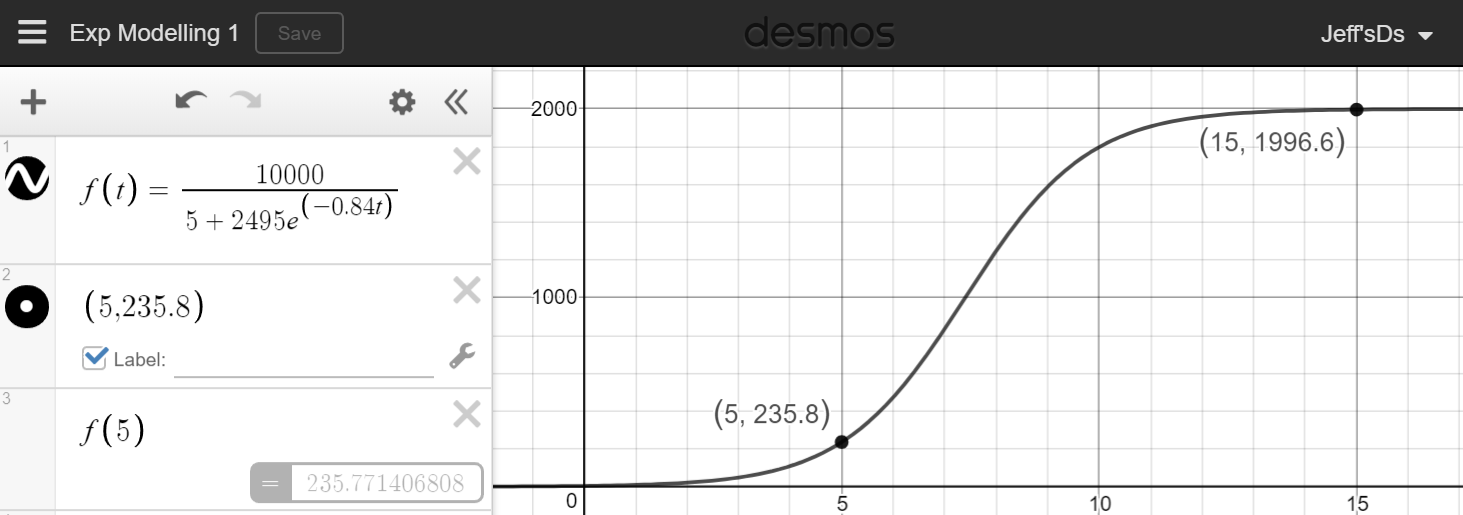
\includegraphics[width=\textwidth]{modelling1}
\end{tasks}

The graph has distinctive characteristics. It starts at a particular non-zero value (when $t =0$) and increases slowly at first then more rapidly. It slows down after a time and levels off because the exponential function in the denominator $ \leadsto 0$ when $t \leadsto \infty $. Graphs with these characteristics are called logistic curves. The particular model is called a logistic growth model. 
\clearpage
\examq\medskip \\In the winter of 2019 the number of people contracting the measles virus grew substantially in the Auckland region. The plot shows the number of confirmed cases with data indicating 546 cases as of August 20, 2019.
\begin{center}
	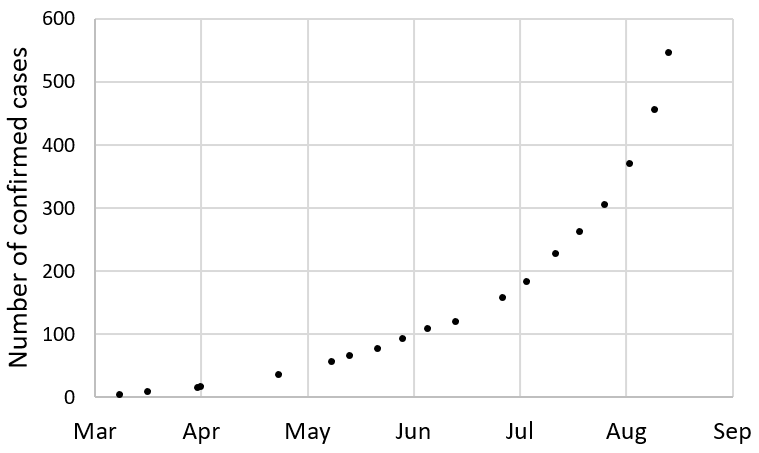
\includegraphics[width=11cm]{measles}
\end{center}
\begin{tasks}
	\task What type of mathematical model (function) would you expect to fit the data?\\
	\[\text{This data most closely resembles an exponential function.}\]
	\task Using Excel, a mathematical formula has been fit to the data:	$\displaystyle f(t)=8.06e^{0.0272t}$ where $t$ is measured in days. How many cases were originally reported?\\
	\[\text{Sub in $t=0$ to find the initial number of cases in the data.}\]
	\[f(0)=8.06e^0=8.06 \text{ cases}\]
	Remember the model is an approximation of the data so it is likely that there were 8 cases to start with.
	
	\task How many days have passed between the initial data point and August 20?\\
	\begin{align*}\text{Solve for \textit{t} knowing that }f(t)&=546\\
	546&=8.06e^{0.0272t}\\
	\frac{546}{8.06}&=e^{0.0272t}\\
	\ln\left(\frac{546}{8.06}\right)&=0.0272t\\
	t&=\frac{4.2157}{0.0272}=154.989\approx 155\text{ days}\\
	\end{align*}
\end{tasks}

%---------------------------------------------------
% Chapter Exercises in a separate file
%---------------------------------------------------
\section{Chapter Exercises}
\subimport{}{3ExpExercises}

% END ----------------------------------------------